%!TEX encoding = MacOSRoman
%!TEX TS-program = xelatex
%!BIB TS-program = bibtex

% --------------------- Start of Document Preamble -----------------------

\documentclass[12pt, oneside]{report} % report is suitable for the long document such as Ph.D thesis with chapters
\usepackage[a4paper, left=1in, right=1in, top=1in, bottom=1in]{geometry} 
\usepackage{fontspec}
\setmainfont{Times New Roman}
\usepackage{pdflscape}
\usepackage{apacite}
%\usepackage[round]{natbib}  % the bibliography
\usepackage{sectsty}
\chapterfont{\centering}
\usepackage{enumitem} % enumerate package
\linespread{2}
\usepackage{amsmath,amssymb,amstext} % Lots of math symbols and environments
\usepackage{graphicx} % For including graphics N.B. pdftex graphics driver 

%----- Adjust the style ----
\renewcommand{\chaptername}{CHAPTER}
\renewcommand{\thechapter}{\Roman{chapter}}
% ---------------------- End of Document Preamble ------------------------

%======================================================================
%   L O G I C A L    D O C U M E N T -- the content of your thesis
%======================================================================
\begin{document}

% For a large document, it is a good idea to divide your thesis
% into several files, each one containing one chapter.
% To illustrate this idea, the "front pages" (i.e., title page,
% declaration, borrowers' page, abstract, acknowledgements,
% dedication, table of contents, list of tables, list of figures,
% included into the document by the following statement.
%----------------------------------------------------------------------
% FRONT MATERIAL
%----------------------------------------------------------------------
% T I T L E   P A G E
% -------------------
% Last updated May 24, 2011, by Stephen Carr, IST-Client Services
% The title page is counted as page `i' but we need to suppress the
% page number.  We also don't want any headers or footers.
\pagestyle{empty}
\pagenumbering{roman}

% The contents of the title page are specified in the "titlepage"
% environment.
\begin{titlepage}
        \begin{center}
        \vspace*{0.5cm}

        \normalsize
        {\bf NETWORK ANALYSIS OF RICE HEALTH SUREVEY DATA FOR CHARACTERIZATION OF YIELD REDUCING FACTORS AND YIELD LIMITING FACTORS OF TROPICAL RICE ECOSYSTEM IN SOUTH AND SOUTHEAST ASIA}

        \vspace*{4.0cm}

        \normalsize
        \bf{SITH JAISONG} \\

        \vspace*{4.0cm}

        \normalsize
        THESIS OUTLINE SUBMITTED TO THE FACULTY OF GRADUATE SCHOOL\\
        UNIVERSITY OF THE PHILIPPINES LOS BA\~NOS\\ 
 IN FULFILLMENT OF THE \\
        REQUIREMENT FOR THE \\ 
        DEGREE OF \\
        \vspace*{2.0cm}
        PH.D OF SCIENCE \\
        (Plant Pathology) \\

        \vspace*{1.0cm}
%        \copyright\ Pat Neugraad 2007 \\
        May 2015
        \end{center}
\end{titlepage}

% The rest of the front pages should contain no headers and be numbered using Roman numerals starting with `ii'
\pagestyle{plain}
\setcounter{page}{2}

\cleardoublepage % Ends the current page and causes all figures and tables that have so far appeared in the input to be printed.
% In a two-sided printing style, it also makes the next page a right-hand (odd-numbered) page, producing a blank page if necessary.
 
%------------Setting the bibliography style --------------



%------------End of the bibliography style ----------------

% D E C L A R A T I O N   P A G E
% -------------------------------
  % The following is the sample Delaration Page as provided by the GSO
  % December 13th, 2006.  It is designed for an electronic thesis.
%  \noindent
%I hereby declare that I am the sole author of this thesis. This is a true copy of the thesis, including any required final revisions, as accepted by my examiners.

%  \bigskip
  
%  \noindent
%I understand that my thesis may be made electronically available to the public.

%\cleardoublepage
%\newpage

% A B S T R A C T
% ---------------

%\begin{center}\textbf{Abstract}\end{center}

% You're not characterizing different environments. They're all tropical, irrigated, lowland rice
%Characterising rice agroecosytems requires knowledge and information of qualitative and quantitative information. One way of gathering data the data necessary for this is through the conduct of surveys. Given the nature of the data, it is not a simple task to analyse and examine in order to derive information and knowledge. One method in particular, network analysis, has been used to explore the observed relationships between the individual elements in a given system. This study is the first known attempt to apply network analysis to the analysis of in-field and household survey data on rice yield limiting and reducing factors. The data will be analyzed and visualized using the proposed network model. I propose to construct a network model using survey data collected from 2009 to 2011 in several sites (Chekempek, West Java, Indonesia; Mekong River Delta, Vietnam; Tamil Nadu, India; and Suphaburi, Thailand) and test the model with data collected from 2012 to 2015 in several cropping seasons and sites (Chekempek, West Java, Indonesia; Red River Delta, Vietnam; Tamil Nadu and Odisha, India; Suphaburi, Thailand). The anticipated results from this research will be helpful for plant health authorities worldwide, in order to design specific strategies for rice pest and disease management and to limit the impacts of these yield reducing factors. 


%\cleardoublepage
%\newpage

% A C K N O W L E D G E M E N T S
% -------------------------------

%\begin{center}\textbf{Acknowledgements}\end{center}

%I would like to thank all the little people who made this possible.
%\cleardoublepage
%\newpage

% D E D I C A T I O N
% -------------------

%\begin{center}\textbf{Dedication}\end{center}

%\cleardoublepage
%\newpage

% T A B L E   O F   C O N T E N T S
% ---------------------------------
\renewcommand\contentsname{TABLE OF CONTENTS}
\tableofcontents
\cleardoublepage
%\phantomsection
%\newpage

% L I S T   O F   T A B L E S
% ---------------------------
%\addcontentsline{toc}{chapter}{List of Tables}
%\listoftables
%\cleardoublepage
%\phantomsection		% allows hyperref to link to the correct page
%\newpage

% L I S T   O F   F I G U R E S
% -----------------------------
\addcontentsline{toc}{chapter}{LIST OF FIGURES}
\listoffigures
\cleardoublepage
%\phantomsection		% allows hyperref to link to the correct page
%\newpage

% L I S T   O F   S Y M B O L S
% -----------------------------
% To include a Nomenclature section
% \addcontentsline{toc}{chapter}{\textbf{Nomenclature}}
% \renewcommand{\nomname}{Nomenclature}
% \printglossary
% \cleardoublepage
% \phantomsection % allows hyperref to link to the correct page
% \newpage

% Change page numbering back to Arabic numerals
\pagenumbering{arabic}
 

%----------------------------------------------------------------------
% MAIN BODY
%----------------------------------------------------------------------
% Because this is a short document, and to reduce the number of files
% needed for this template, the chapters are not separate
% documents as suggested above, but you get the idea. If they were
% separate documents, they would each start with the \chapter command, i.e, 
% do not contain \documentclass or \begin{document} and \end{document} commands.

%======================================================================
% INTRODUCTION
\chapter{INTRODUCTION}
%======================================================================
%=========================
%INTRODUCTION
%=========================
%\section*{Introduction}
\addcontentsline{toc}{chapter}{Introduction}
% 1. Why are you talking in past tense in your opening sentence? I already commented about being consistent in your verb tenses.
% 2. Sentence 2 should be part of sentence 1.
% 3. "at irrigated areas" is awkward. It should be "in irrigated areas"
% 4. No "," after "approximately".
% 5. Your punctuation in the entire para is a shambles.
% 6. This para is out of place. It needs to be in your M&M for the section.

Pests and diseases to global rice production are significant yield reducing factors. \shortciteA{OERKE:2006ct} estimated that rice pests potentially caused losses around 37 percent of global rice production. Additionally, future rice production will need to grow by 2.4 percent per year in order to meet the demands of a growing population \shortcite{Ray:2013by}. Addressing these yield-reducing factors is essential for food security not only in rice consuming societies, but also for other societies societies globally.

% 1. The sentence starting with "A survey" doesn't need a ","
% 2. Did Serge just imply or did he state that management strategies should be developed according to patterns?
% 3. Last sentence is a bit unclear. Revise.

Nowadays, developing the strategies of pest and disease management takes into account sustainability, production efficiency, and environmental protection \cite{Mew:2004kh}. To achieve this, interactions between pests and human activities must be studied. A survey may provide the necessary data, and adequate methods for analyzing survey data can produce preliminary information on their behaviors including major interactions \shortcite{savary1995use}. \shortciteA{Savary:2000vr} concluded that the observed injury profiles (i.e., the combination of disease and pest injury that may occur in a given farmer’s field) were strongly dependent on production situation. It was implied that pest management strategies should be developed according to the patterns of cropping practices, and production situations. However, interactions among pests, cropping practices, and environments are difficult to elucidate. Moreover, most previous analytical techniques can not be used to reveal their changes across locations or time, which they are important to design the strategies of pest management. 

Network analysis provides a promising tool for revealing the interactions among entities within a complex system. It has been applied for many branches of science (e.g., social science, computer science, biology). A network model is an abstract model composed of a set of nodes or vertices and a set of edges, links or ties connected to the nodes. Nodes usually represent entities and the edges represent their relations. For example, an ecological network of a food web presents nodes as species \shortcite{krause2003compartments} and edges as ecological relationships, or consider a social network of students in the school present where nodes are students and edges are friendships \shortcite{moody2001race}.

%-----------------------------
\section*{OBJECTIVES}
\addcontentsline{toc}{chapter}{Objectives}
%----------------------------

% 1. Confused. I thought that this was basically a proposal for your disseration. Why are your goals written in past-tense? Are they not present or future, you've not completed the work yet, unless I'm unaware.
% 2. You don't need commas before every "and", I've seen this at least twice in this section alone
% 3. Third objective, different levels of yield gains? I'm unclear on what you mean here. Yield gains have a very specific meaning, how are you studying them?

My overall objective was to develop network approaches, and apply them to analyze crop health survey data. My first objective for this research was to develop the network model based on crop health survey data and characterize relationships among components of injuries and cropping practices. My second objective was to compare the differential relationships of network models under different seasons or locations. The third objective was to compare differential patterns of their relationships at different levels of yield gains.

% 1. Again, verb tense. Is this work that you've already done? If so, why are you submitting this to the graduate school?
% 2. Grammar in first sentence and second sentence

Once network models based on crop health survey data were constructed, they can be helpful for plant health authorities, and the people who related to crop protection especially for rice. The models support them to design specific strategies for rice pest and disease management and to limit the impacts of these yield reducing factors.  

% eos


\chapter{REVIEW OF LITERATURE}
%====================================
% introduction of literature review
%===================
\section*{Introduction}
%==================
\label{ch:intro}

The applications of network analysis have increased exponentially over the past two decades in various disciplines. Even though documented applications of network analysis in plant pathology are still relatively sparse, network applications in the social science, systems biology and ecology have been increasingly found. \shortciteA{Shaw:2014cka, MoslonkaLefebvre:2011fo, Jeger:2007tn, windram2014network} presented useful concepts and methods of network analysis in the studies related to plant pathology. I review the empirical works that exist and argue that network analysis is a promising approach for exploring the questions in the context of plant pathology.

This chapter contains four sections of review of network analysis and its applications. In the first sections, I introduces a brief overview of the concepts and methods of network analysis. I then discuss the new dimensions of network analysis that are not found in other approaches. In the first two sections, I provide an overview of key of network concepts and place network analysis as a methodology within the broader toolbox of methods commonly used in biological studies.
  

In the third section I scope network analysis  into the current applications of plant pathological research, particularly in plant disease epidemiology and molecular plant pathology, in which network analysis has been broadly applied, and increasingly documented. It provides fruitful tools for visualizing, analyzing and understanding complex relationships in the studies of plant disease. For instance, network models of genes or proteins pertaining plant defense mechanism and network models revealing spatial distribution of plant disease through trade networks were reviewed by \shortciteA{windram2014network} and \shortciteA{Shaw:2014cka} respectively. 

The last section presents analytical techniques and strategies to apply network analysis for studying pest management. It introduces three strategies of network applications, which are developed and applied in the studies of systems biology and ecology, and concludes the brief discussions of potential applications to the studies of crop heath management that have yet been undertaken.

\section*{PartI: Network Analysis}
%==========================
\label{ch:partone}

\subsubsection{Introduction to network analysis}
Network analysis is applied for determining relationships between elements of interest. It offers toolkits for visualizing data in a network model and measuring its properties, and network thinkings \shortcite{PROULX:2005hx}. It been widely used by various branches of science, such as social science, ecology, biology, computer science, and many others to study the interactions between elements, e.g., the relationships of students in school \shortcite{moody2001race}, species in food webs \shortcite{krause2003compartments}, interactions of genes or proteins in cells \shortcite{guimera2005functional}, or the connections of computer in the network \shortcite{pastor2001epidemic, newman2006modularity}.

\shortciteA{newman2003structure} loosely categorized four types of networks based on different complex data. The first category is social network, representing sets or groups of people forming some patterns of contacts or interactions between them such as the patterns of friendship or business relationships. Analyzing the structure of whole social entities gives us the perspectives from a social network, which enables us to explain the patterns observed. \shortciteA{moody2001race} analyzed the social behaviors in high school students using social network approaches. \shortcite{Kasari2011s} applied network analysis to compare the social relationships and friendships between children with and without Autism spectrum disorder (ADS). The second type of network is an information network or knowledge network. The classic example of this network is the network of citations between academic papers \shortcite{newman2003structure}. The articles cited other papers, which have related topics. They formed a citation network that has vertices as articles and direct links as citations. The citation network visualizes the structure and the movement of the information. The third category, technological network, is object connected network, or man--made network which represents a physical connection between objects. This network is mostly applied for illustrating physical structures and systems such as the electrical power grid, the connections of rivers, transport systems, etc. The fourth category of network is a biological network. It represents the biological systems such as genes to genes, genes to protein, protein to protein interactions, which enable biologists understand the connections and interactions between individual constituents including genes, proteins, and metabolites at the level of the cell, tissue and organ to ultimately describe the entire organism system. Biologists use biological networks in various branches of biology at different levels (from a single molecule to an entire organism). For example, \shortcite{yang2014gene, barabasi2004network} studied in the patterns of gene expression in different conditions and different types of cells (normal cells and cancer cells) in order to characterize the genes that change and do not change following the particular conditions; \shortcite{freilich2010large} applied a molecular ecological network analysis to study the communities of soil microorganisms. Networks revealed the complex relationships between microbial species in soils and their communities. Moreover, network analysis enables ecologists to understand ecological properties and predict the ecological roles of species in a soil ecosystem. Although the application of each type of network approach varies, all four categories of networks share a common empirical focus on relational structure and a similar set of mathematical analysis. 

% add more the ecological studies related to plant disease
In plant pathological studies network analysis can be the powerful tool to study plant disease epidemics. \shortciteA{MoslonkaLefebvre:2011fo} showed the  the potential for the use of network analysis in plant epidemiology. Network analysis can reveal the dynamics of the disease spread. The theory and tools of network analysis support plant pathological studies. \shortciteA{MoslonkaLefebvre:2011fo} reviewed the studies related to plant disease which applied network analysis. Networks applied in the studies of plant disease are generally similar to ecological studies. In plant pathology, most network analysis is used in molecular plant pathology as a model of the interactions between genes and/or proteins, and other cellular constituents contributing to host plant resistance or pathogen infection. Spatial analysis 


\subsection*{Concepts, principles, and methods of network analysis}

A network represents relationships between of elements of interests, which is defined by links (edges) among nodes (vertices). Nodes can be units of interests or studies, and links represent interactions between nodes. Network analysis aims the association among nodes rather than the attributes of particular nodes. In network analysis, networks are defined as any set or set of links between any set or sets of nodes.


Network analysis follows three principles. Nodes and their behaviors are mutually dependent, not autonomous; links between nodes can be channels for transmission of both material (for example, money, disease) and non-material (for example, information, knowledge, relationship, interaction) and; persistent pattern of association among nodes create structure that can define, enable, or restrict the behavior of a node.  

Network models have two different organizational structures depending on the goal of the representation and analysis \shortcite{borgatti2013analyzing}. Flow models view the network as a system of pathways along which things flow between nodes. Analysis of flow models can, for example, identify which nodes in the network are more active, or which ones are more powerful. Flow models are good for evaluating processes, as was shown in these reviews of plant disease spread \shortcite{Jeger:2007tn, Shaw:2014cka}. Architectural models tend to focus on the structure of the network, seeking to discern whether specific structures lead to similar outcomes, or whether actors in similar network positions behave in similar ways. Ecological applications related to the ecology and spatial structure of ''community'' tend to be organized and analyzed as architectural models. For example, \shortciteA{Faust:2012dk} studied the networks of soil microbial interactions. Network models describes how microbial populations change over time, which will require the use of dynamic models of microbial communities. Beyond these basic principles, network analysis enables the calculation of structural properties of nodes, groups, or the entire network.

\textit{Measuring network properties}


A network is made up of nodes and links from relational data. It is constructed from adjacency matrix, which is obtained from analysis using metric algebra techniques. The row and column headings for an adjacency matrix are identical, listing the names of the components involved in the network. In the simplest case, the cells of the matrix are coded with ''1'' if an link exists between the node or ''0'' if no edge exists. However, a link can be valued. Value indicates a characteristic of the relationship that the research has quantified. The values may be binary, such as whether two friends recognize each other, or variable strength, e.g., the number of mutual friends between two friends. Network link need not to imply positive or cooperative interaction; they can also be negative or competitive interaction between two individuals.    


The distribution of links in a network suggests two important structural characteristics: centrality (importance) of nodes in the network and division of the network into subgroups. Variants of centrality in a network include degree, closeness, and betweenness. Degree centrality of a node is the sum of the value of the links between that node and every other node in the network. This measure tells us how well-connected a particular node is to the other nodes. Closeness centrality is calculated using the length of the path between a node and every other node. This measure could estimate the time required for information or resources to propagate to a given node in a network. Betweenness centrality corresponds to the number of paths in the network that pass through a particular node, and therefore measures the dependence of a network on a particular node for maintaining connectedness \shortcite{Toubiana:2013cv}. \shortciteA{Deng:2012do, newman2003structure, Toubiana:2013cv} are recommended references for descriptions of the theory and uses, as well as the formal calculation of these measures.


 %==========================
\section*{Part II: The dimensions of network analysis unlike other approaches}
%==========================
\label{parttwo}

%There are four key points to consider in network analysis :
%1) how does it differ from traditional approaches to social science research; 
%2) how does it relate to those traditional approaches; 
%) how are networks are constructed, manipulated and measured; and 
%4) what is value of network offers beyond traditional approaches.

With an increasing trend towards a systems level perspective in the science, away from the reductionism that characterized much of the previous century \shortcite{kolaczyk2014statistical}, the development of network analysis challenges conventional approaches to uncover the complex patterns of interaction or relationships. 

The difference of network analysis from conventional approaches is that it involves different methods of analysis. 
Network analysis models the relational data, and measures various properties of network. A challenge of network analysis is the consideration of the properties of interactions  between elements in the system, which interactions are assumed that they are dependent on each other. That is, when element A has a relationship with element B, the relationship is not only considered to be independent of element A and B, but also relationship of element A and B to be independent to other element. Unlike network analysis, traditional research methods consider attributes such as variables in a wide variety of statistical analyses, these methods are sometimes referred to as variable analysis \cite{scott2012social}.

As objects for representing interactions among elements of a complex system, network graphs are primarily focused in network analysis. Interactions or relationships are represented as edges in networks. They present only when interactions are exist between nodes. Moreover, network concepts place nodes in rational distance according to the level of relationships. For example, to visualize the strong relationship of A and B, network places the node represented A near the node represented B. Here is the new dimensions network of visualizing interactions or relationships.
 
Extending from considering the interaction of two nodes, network graphs illustrate nicely the connections. when node A relates to node B, and to the node C are found relationships, the network graph is able to visualize the connection between node A to node B, and to node C. This pattern, so-called "betweenness", potentially is useful to represent what the important node is in network graph because node A has high connectivity and is a connector between node B and node C. For example, In protein-protein interaction (PPI) network, proteins with high betweenness have been termed "bottlenecks", for their role as key connector proteins with essential functional and dynamic properties \shortcite{barabasi2011netmed}.

The heart of network study is structure; network processes replace vertices and edges in rational spaces depending on the selected graph layout methods. The network structure enable scientists to study interactions with behaviors and attributes of pairs of vertices. Networks would reveal the groups of vertices, which are closely related or similar to each other. This is also similar to the basis for the cluster analysis. For example, if the employees of the same company may share similar attributes such as location or educational background and they are close in network. When the relationships are simple and the differences in node attributes are clear, the conventional analytic approaches such as cluster analysis, principal component analysis, correspondence analysis are sufficient. However, when relationships are complex or vertices attributes are more nuanced, clear answers using conventional analysis may prove elusive. Network analysis offers a tool to help researchers disentangle some of the relational complexities.

\section*{Part III: Network and botanical epidemiology}
\label{ch:partthree}

Recently, a broad expansion in the use of network analysis has occurred across many disciplines over the past decade, and several researchers have evaluated the impact and potential of network approach on their respective disciplines. Networks are considered into the studies of plant pathology. \shortciteA{MoslonkaLefebvre:2011fo, Jeger:2007tn} provide insightful analysis of the reasons why network analysis is useful in the study of plant pathology. Given the generality and flexibility of the approach, network representations can be used at a variety of levels in plant pathology, from gene expression during host–pathogen interactions, to the development of plant epidemics among fields, farms, and landscapes and to trade movement of plants infected by pathogens or infested by insects among regions and countries. 

Networks can provide such a unifying framework. There are two fields in the literature relevant to plant pathology particularly strong growth where network analysis has been used or has significant potential to augment traditional analysis methods. The first is plant disease epidemiology, which investigates questions related to plant disease spread. The second is plant molecular biology, which investigate question related to biological network. Here I briefly review these two theme and identify a few studies that have begun to integrate them.


\subsection*{Using Network analysis to understand plant disease spread}

The idea of plant disease spread is that the probability of infection embedded in the connection or the contact patterns between susceptible/infected plants, and it forms as the networks. In network theories and analysis,  plant disease spread and establishment were able to be modeled in directed, indirected networks using scenarios concerning networks \shortcite{Jeger:2007tn}. The disease is started at a single node, and which will connect to others node when they are infected over time with a certain probability of transmission. In turn, already infected nodes will be infected at the next time step depending on their infection status and on a certain probability of persistence. The probability of infection transmission is the same for all connections in a given network replicate. The probabilities of persistence and transmission define an epidemic threshold, which is independent of the starting node of the epidemic, and will influence to the structure of network. 

Network analysis includes models developed specifically to answer questions related to flows of information and structures of connections through networks. Tracing information flows through a trade network can expose critical gaps or inefficiencies that may contribute to plant disease control policies as classified by. Routes and network nodes of transmission were studied for trade transmission. \shortciteA{xu2009spatio} revealed \textit{Phytophthora ramorum} epidemics in the horticultural trade network. For P. \textit{ramorum}, the epidemic networks in the horticultural trade and the seminatural landscape showed independent systems. Combining genetic network analysis and data on trace forward and trace back on movement of plants nursery trade supported to identified confidentially P. \textit{ramorum} migration. From this approaches, it was clear that pathogen was introduced originally from nurseries, which P. \textit{ramorum} populations in nurseries are genetically ancestral to all Californian forest populations.


Network models developed enable the researcher, policy makers or related person to identify or predict what entities play the key role in the network. In trade network. network analysis suggests broadly that it would be sensible to place quarantine efforts on hubs or on connections between major hubs. However, wherever effort is placed, a disproportionate increase in quarantine effort is needed to keep the rate of flow of pathogens across trade links constant as the trade through links increases \shortcite{dehnen2010structural, MoslonkaLefebvre:2011fo, Shaw:2014cka}. For instance, trade network of plants and plant products across the world and within countries give the picture on how to be able to control the flow of pathogens. The strategy should be designed by focusing on links to and from hubs, nodes which have high degree of connectivity would increase efficiency to achieve control plant pathogen spreads.  To cope with increasing volumes in trade of potential infected plants, this insight may be very helpful for plant heath authorities target at the traders who have high connection activities or find the major pathways. The control of disease or quarantine can be made more efficient and effective.

\subsection*{Using Network analysis to understand molecular plant pathology}

The development of bioinformatics and biostatistics method and increasing number of biological data have influence to the "new" biology \shortcite{rose2007new}. Recently, the representation of biological systems by networks (graphs) is commonly applied in biology to analyze the systemic interplay of biological components. When the systems (biological systems, for example) are very large and have many fractions of unknown contents in there, top-down approaches are often applied \shortcite{windram2014network}. To apply network analysis attempts to infer properties of the system (such as network structure or parameters that can capture the system dynamics range interactions over time) from large scale biological data sets in order to identify interesting features that may be tested using more targeted experiments. 

Network analysis offers tools to visual the myriad information. \shortciteA{wu2007gene} built a network from the gene-for-gene relationships between rice and various avirulence genes of the pathogen \textit{Xanthomonas oryzae}, which its nodes represented isogenic lines of rice and links are connected if they share genes with high resistance (with respect to avirulence genes). This network can help rice breeder to identifying particularly promising genes for developing host resistance to pathogens. General presentation, such as genetic maps, frequency distributions, etc. are also equally value, but network models are clearly able to provide an overview of relationships in a given system. 

The network approach focuses on components of network structure that cannot be created from observing individual nodes alone. Recently, biologists have attempted to understand the nature and consequence if biological complexity using network analysis to understand the network structure of biological. For instance, networks can be constructed from available data for a certain plant pathogen from multiple locations/hosts based on the similarity among the pathogen strains. \shortciteA{MoslonkaLefebvre:2011fo} showed the good examples, which are co-occurrence network of the \textit{Phytophthora ramorum} infected plant genera different environment.The networks may be helpful in identifying host taxa playing a important role in spreading a certain disease in the semi- natural environment, in crop plants, and plants in the trade.

Network analysis can contribute to our understanding of biological mechanism and interaction, and influence by analyzing the network composition and interdependent relationship (network structure) of elements in biological processes. Granted, network analysis is not needed for simple assessment of network composition; that is, to measure the relative levels of key components in the processes. However, what it does offer is the ability to identify and compare the structural positions of individuals and their relationships. Systematically and simultaneously analyzing network composition and structure provides much deeper insights in holistic view. Plant-pathogen interaction network by \shortciteA{mukhtar2011independently} revealed the complicated  that a large number of novel Arabidopsis protein-pathogen effector interactions, provided evidence that pathogen effectors target a limited number of host immune proteins, and demonstrated that effectors from very distantly related pathogens interact with the same host proteins. \shortcite{Lu:2013hga} construct the network of soil fungal community. They compare the fungal networks with different condition, yield-invigorating and yield-debilitating soils under prolonged potato monoculture. from this comparative network, the result showed that \textit{Sordariales} and \textit{Hypocreales} were major affected phylogenetic group. Network analysis enables the identification of elements and their relationships that need to be bridged to overcome problems of relational complexity.

%==========================
\section*{Part IV: Application of Network analysis to study of Agro-Ecosystems}
%==========================
\label{ch:}

The usefulness of network analysis related to applications of plant disease management. I mentioned in the previous topic falls into two broad types of applications. The first is network application in landscape plant disease epidemiology  . This applications tend to be more flow oriented, while the second type of networks related to plant molecular biology  tends to be more emphasized in the structure. In both of these applications the literature shows a progression tend to from theoretical to empirical approaches over time \shortcite{MoslonkaLefebvre:2011fo}. For this chapter I give the literature related to specific applications as the third type of plant disease studies, which network analysis is used for and focus on analyzing plant pathosystem. 

The network theory applied in plant pathology would broaden windows of opportunities to plant pathologists to understand the causality of plant disease epidemics. Diversity is primary causes, for example to shape plant disease epidemics. \shortcite{MoslonkaLefebvre:2011fo} claimed that networks is a tool to examine the relationships between plant diversity and ecosystem susceptibility to plant pathogens, and networks also show the capability of revealing system perturbations, which we can see what the difference between system with and without interference(e.g. plant pathogen introduction or pesticide use), so they will enable us to predict the consequences in order to improve the sustainability of agriculture.

Alternatively, network analysis can be implemented to analyze plant pathosystem. To maintain the agricultural sustainability, plant pathologists need to develop a more holistic approach to crop protection. It is pathosystem analysis, which considers the various pests, including disease, insects and weed that affect a crop, and cropping practices, and also determines their interactions. A survey may provide the necessary overview of the pathosystem; adequate methods for analyzing survey data can produce preliminary information on its behavior including major interactions.In this context, surveys can be considered as part of a systems approach. use the survey data to analyze the characterization, the dynamics or the behavior of pathosystem.

Traditional approaches are found limitation in analysis the data with high heterogenouse and dimensionality. The survey data have that format. Various statistical approaches are used to reduce dimensions and extract major feature, including principal components, correspondence analysis The survey generated both of quantitate and qualitative data. In multivariate statistical analysis, traditional methods analyzing the data set which contained both type of variable are principle component analysis, correspondence analysis etc. Correspondence analysis normally have been picked up to analyze the survey data related to plant disease \shortcite{Avelino:2006ie, savary1995use, Savary:2000ws}. Briefly, there are two main stages. The first stage is to convert the quantitative variables into classes by using cluster analysis, then perform Chi-square test to prove that the class of variables are independence. The number of classes and their limits could be fixed in line with critical thresholds known beforehand \shortcite{savary1995use}. The second stage is to perform correspondence analysis. The limits of the categories of explanatory variables used in the segmentation played the role of decision thresholds. because this methods has a limit, which there is no solid role of choosing category limits, \shortciteA{Avelino:2006ie} claimed that if categorized variables have influence experimentally or particularly to a large degree, those limits had been chosen. The logic of the results obtained tended to back the choice made. Although no general rule can be imposed when choosing category limits \shortcite{savary1995use}, it is necessary to validate them experimentally, particularly if they have to influence decision making, such as the decision to carry out chemical control.
 
Like multivariate statistical analysis, network analysis are equipped with a set of tools to analysis the large datasets with homogenous and heterogenous. In biological point of view, correlation-based networks are commonly used for generating biologically meaningful hypotheses and for gaining novel insights into the complex relationship \shortcite{Toubiana:2013cv}. Expending the key role of the classic disease triangle (host–pathogen–environment), plant pathosystem profoundly conserved that classic role. Moreover, human and human activities have possibly additional factor, and strongly influence plant disease epidemics. For plant disease control (may included pests) to succeed, the holistic view of the interconnectivity of components causing plant disease development and their influences is critical. This section reviews the challenges of network application for analyzing plant pathosystem that have not been discussed previously in this literature. These challenges discussed fall into three concept of network analysis.

\paragraph{Concept 1: Networks are generated from multiple pairwise relationships of data through the statistical approaches.} 

The networks are inferred from the assumption of interaction and influence between components generated from statistical relation in the observed data. Interaction between two elements involved falls into one type of interaction in someway. Otherwise, there will not have interaction. In microbial association network, the relationships can be predicted from determination to co-occur or show a similar pattern over the multiple samples or time. Also similarly in context of protein-protein interaction, for example, if protein A induces expression of protein B, then expectedly levels of protein B are high whenever levels or specific molecular states of its activator A are high. The reverse of this logic is that statistical correlation between protein states indicates a potential interaction between them.

A relationship between two entity of network can be predicted by means of two group of network inference methods; Pairwise relationships: similarity-base network inference and Complex relationships: regression- and rule-based networks. 

There are serval techniques to determine the similarity between variables depending on the biological question to be answered. Mainly using either Pearson's or Spearman's correlations for data \shortcite{qin2010human, barberan2011using} and the hypergeometric distribution for presence-absence data \shortcite{freilich2010large}. Another popular similarity-based network inference methodology is local similarity analysis (LSA) \shortcite{Faust:2012kq}, which can detect similarity between shifted abundance profiles and is therefore frequently used to build association networks from time series data. In an interesting alternative approach, Pearson correlation thresholds are determined using random matrix theory \shortcite{Deng:2012do}. These approaches should be evaluated, and compared which approaches are good evaluation. Pairwise relationship does not always mean that there is a biological relations for two compared variables because they may be influenced by other variables in the system. Regression- and rule base networks are also applied, especially in ecology fields to infer complex interactions \shortcite{Faust:2012dk}, and there are other techniques such as mutual information analysis must be applied \shortcite{zhang2005general}. 

\paragraph{Concept 2: Networks are not static, but dynamic according to the given data and environments.} 

Networks can dynamically respond and adapt to the internal state and external signals \shortcite{Peer:2011jd}. As the internal state, backgrounds of nodes have big influence to the structure and behavior network, and give rise to significant difference across individuals. Backgrounds are included information about where the data are from. The different sources and different times collecting the data strongly determine the network behaviors. 

Exogenous signals such as nutrients, chemicals, environmental conditions, affect to networks. Networks can be constructed from different sets of data (e.g., from different locations, sources), structural properties can be used to determine the differences between the networks \shortcite{Subramanian2005}. Protein-protein interaction network models can vary significantly between different condition  \shortcite{windram2014network}. Comparative network broadly are construct for comparing the series of parameters related to network topologies under different situation. For examples, in a soil microorganism community, the context can profound impact on how the communities at difference between different types of soil. \shortcite{Lu:2013hga} compared the fungal communities of yield-invigorating and -debilitating soils from prolonged potato monoculture. Fungal network of healthy soil showed high connectivity and  soil organic matter are influence to connectivity of network of healthy soil, whereas degree of connectivity fungal networks of disease soil relatively low, and ammonium nitrogen and electrical conductivity were related to the connectivity of this network.

\paragraph{Concept 3: Differential networks focus on the changes.} Challenging to network models by comparing networks across multiple environment is valuable. Networks can response differently under various environments or with external signals. They can be more simplify by focusing on key components and capturing only the essential components differently responding between environments which they play a key role in the modeled response \shortcite{Peer:2011jd}. Networks are examined by adding or depleting some variables. This allows predicting interactions or components that change following the changed structure of networks. 

Data-driven computation, In silico network inference, can generate network very similar to those identified using experiment technique, which it can be used to identify the additional components interacting with the altered nodes, qualify and qualify the network after encountering perturbation. \shortciteA{mukhtar2011independently} showed clearly evidence that this computational prediction with experiment data can obtain novel opportunities for plant defense network modeling. 

\section*{Summary}
\label{ch:summary}

This literature has presented a brief introduction to the concepts and methods of network analysis. It has attempted to position network analysis as both a unique perspective and unique methodology with respect to analytic approaches and methods commonly used in plant pathology. Building on this foundation the literature ten identified two branches of plant pathology which network analysis has been identified as particularly useful, and examine theses. I concluded that network analysis has the potential to advance and operationalize certain aspects of plant disease epidemiology which mostly dealing with multidimensional data. In particular, network analysis has potential to help plant pathologists visualize, measure and document sources of epidemiological phenomena and to identify specific components contributing these situations.  

Having developed a basic understanding of network analysis from both methodological and theoretical perspectives, the literature proceeds to review network concepts and methods in general. Roughly, Networks have four types, social network, information, technology network, and biological network. Even though, four types of networks are described and applied in different context. They share a common empirical focus on relational structure and a similar set of mathematical analyses. Node or vertex, link or edge. Network models are cable of presenting unique values, which are traditional approaches can not present. 

Network concepts and methods are mainly found in the literature on two broad studies particularly in plant disease application. On the issue of understating plant disease spread, the literature suggests that further use of networks analysis concepts and methods enable us the holistic understand the flow of disease spread, and improve the implementation of plant disease policy. The literature of molecular plant pathology offers two challenge of network application. The fist challenges is to apply network to model large and complex biological dataset. Another challenge is consideration network structure to understand biological system. Emergent properties of network structure influences  may be identified, measured and analyzed to yield better explanations of the experiments being observed.

While documented plant pathosystem studies using network analysis remain quite sparse, Using network analysis concepts and methods augment existing approaches and provide tools for exploring the relations dimensions, which has been widely acknowledged as influential but difficult to measure using traditional methods. This chapter claimed network analysis is ideally suited with high dimensional data, such as survey data, which is commonly used in the studies of plant pathosystem. With concepts and approaches giving generality and flexibility, networks can potentially model plant pathosystem as a subsystem of agroecosystem. Three concepts of network analysis are introduced to challenge the network application for system analysis in plant pathology. Addressing the challenges identified in this paper represent first steps in plant pathology  to take advantage of these new opportunities.



%======================================================================
% Materials and Methods
\chapter{MATERIALS AND METHODS}
%======================================================================
%=========================
% Materials and Methods
%=========================

% Your not including yield in your analysis? Seems to be a big reason for this work. Why is it not included?
This research will use data collected from surveys of irrigated lowland rice growing areas in South and South East Asia to examine relationships between the injuries caused by pests and diseases, cropping practices (\textit{e.g.}, rice variety grown, crop establishment method, fertilizer and chemicals applied). Their relationships will be constructed and analyzed through network analysis. I will develop and apply suitable methods of network analysis to characterize the associations of injuries and cropping practices. The resulting network of associations of injuries and cropping practices will thus provide a starting point for further investigations of their relationships (\textit{i.e.}, characterization of relationships of cropping practices and injury profiles related to yields, comparison of networks under different production environments or examination of networks at different levels of yield gains). 

In the following, I present three distinct network analysis approaches: single-network analysis, differential network analysis, and dynamic network analysis. These three approaches will answer different questions. I will apply single-network analysis to the data from all fields surveyed for identifying patterns of interactions between injuries and cropping practices and key components (\textit{e.g.}, most connected variables). Second, differential network analysis will aim to uncover similarities and differences of networks constructed from the different data sets (\textit{e.g.}, dry season versus wet season). Dynamic network analysis, the third type, will be applied to study how networks changed under at least two different aspects of an evolving complex system. Here, I will focus on dynamic networks by dividing farms into different levels of yield attained. 

\subsection*{Crop health survey data}
\addcontentsline{toc}{subsection}{Crop health survey data}

% how many farmers' fields were surveyed?
Crop health survey data were collected through surveys of farmers' fields (approximately 800) from 2010 to 2015 for both wet and dry seasons in different production environments across South and South East Asia representing irrigated lowland rice growing areas West Java, Indonesia; Mekong River Delta and Red River Delta, Vietnam; Tamil Nadu and Odisha, India; and Suphanburi, Thailand. The survey protocol described in the IRRI publication, ``A SURVEY PORTFOLIO TO CHARACTERIZE YIELD-REDUCING FACTORS IN RICE'', \citep{Savarysurvey2009} was used for data collection. The variables collected included environmental attributes, patterns of cropping practices, crop growth measurement and crop management status assessments, measurements of levels of injuries caused by pests, and direct measurements of actual yields from crop cuts. The data collected can be classified into three groups: cropping practices, injuries, and actual yield measurements.

Cropping practice data included information on the type of rice variety (traditional variety, modern variety, or hybrid rice), crop establishment methods used (direct seeded or transplanted rice) and were collected as categorical data. Pesticide usage (molluscicide, herbicide, insecticide and fungicide) were collected as discretized data, and accumulated organic, synthetic fertilizers were collected as continuous data.

Injury data were gathered on diseases, insects and weeds observed at two development stages of the growing crop: active tillering and active ripening. While injuries due to diseases and insects were specific to species (or species groups), information on weed infestation was the area covered by any weed species, either above or below the crop canopy. Information pertaining to injuries was collected in the form of number of injured organs (tillers, leaves, and panicles), which later was made relative to the corresponding total number of organs present in the sampling units; 12 hills per field for transplanted rice crops, or 12 $\times$ 10 cm quadrat for direct seeded rice. As for weed infestation, the proportion of soil area covered at two levels of the crop canopy (below or above) was assessed in three points in the field of 1 $mathrm{m}^{2}$ each. For this purpose, two types of injury indices were used: area under injury progress curves (AUIPC) or maximum level at any of the two observations, depending on the nature of the injury. Injuries which is occurred on tillers, hills and panicles were quantified as maximum level, whereas juries which occurred on leaf were quantified as AUIPC. The AUIPC was calculated by the mid- point method using the following equation: $\mathrm{AUIPC} = \sum\limits_{i=1}^n\frac{1}{(x_{i} + x_{i-1})(T_{i} - T_{i-1})}$, where $x_i$ is percentage (\%) of leaves, tillers or panicles injured caused by pests (e.g., leaf blast, leaf folder), percentage (\%) of weed infestation (ground coverage) at the \textit{i}th observation, $\mathrm{T}_{i}$ is time in rice development stage units (DSU) on a 0 to 100 scale (10: seedling, 20: tillering, 30: stem elongation, 40: booting, 50: heading, 60: flowering, 70: milk, 80: dough, 90: ripening, 100: fully mature) at the $i$th observation where $n$ is total number of observations.

% Corrected for tense.
% yield data weren't "estimated" they were measured.
% corrected for clarity.
Yield data were measured from three randomly selected crop cuts that were 5 $\mathrm{m}^{2}$ (2 $\times$ 2.5 meters) and dried to 14\% moisture content and weighed.

\section*{Single network analysis of crop health survey data}
\addcontentsline{toc}{section}{Single network analysis of crop health survey data}

%% 1. First sentence is unclear.
Cropping practices and injury profiles network will be constructed from the pair--wise correlation matrix between any variables of injuries (insect injuries and diseases) and cropping practices (fertilizer usage, pesticide applied,rice varieties and crop establishment methods). The edges of the network will correspond to the degree of correlation between two variables. A standard measurement of correlation between two variable $x$ and $y$, $cor(x,y)$, where values are  between -1 to +1 depending on the level of relationship. $cor(x_{i}, x_{j})$ is equal to -1 when there is a decreasing relationship between $x$ and $y$, and +1 when there is a increasing relationship.

To identify the most suitable pairwise correlation methods, I will evaluate four correlation based measures, Pearson's correlation, Spearman's rank correlation, Kendall's correlation, and biweight midcorrealtion. The statistical programming language \textsf{R} will be employed to compute pairwise correlation \citep{R:2014a}. The \texttt{cor.test()} function will be applied for generating a correlation matrix, which describes the pairwise correlations between variables. This function allows users to choose types of correlation measures to perform such as Pearson's correlation, Spearman's rank correlation and Kendall's rank correlation. To compute biweight midcorrelation, I will apply the \texttt{bicor()} function from the \textbf{WGCNA} package \citep{Langfelder:2008bd} in \textsf{R}. 

% p-values should be determined or calculated?
When a correlation matrix is created, the next step is to construct the correlation based network. However, $p$~values should be determined because correlation will be considered if    its $p$~value is less than $p$~values at considered significant (\textit{e.g.}, 0.01, 0.05). As with issues previously mentioned above, $p$~values must be adjusted for multiple testing. Using a Benjamini-Hochberg adjustment or Bonferonni correction is recommended by \citet{kolaczyk2014statistical}. The \texttt{fdrtool()} function of \textbf{fdrtool} R package can calculate adjusted $p$~values. These values are compared to a standard 0.05 significance level. The final correlation matrix contains pair-wise correlation coefficients, which have adjusted for $p$~values lower than 0.05 significance level.

% 1. The first sentence after that is still unclear.
The \textsf{R} packages: \textbf{igraph} \citep{Csardi:2010wx}; \textbf{qgraph} \citep{qgraph}; \textbf{statnet} \citep{statnetpackage} and \textbf{network} \citep{networkpackage}; and \textbf{sna} \citep{snapackage} will be used to construct and analyze network models.

%====================== Comments===================
% why knowledge of biological literature? Why not a good understanding of the biological system that you are monitoring? I think that's more essential and useful
% models cannot reveal knowledge, look up the definition of knowledge. It does not apply here. What do you really mean because it can not be knowledge?
% first sentence, all of them what?
% based on what study? Our study? Who is "we"? This is YOUR research. If anything it should be "based on my study" but I'm not clear as to what study you refer to here. Who are the "we" that are suggesting? You're the only author on this manuscript. It's your dissertation. There is no, our, us or we. It's only my, me, I here.
% Is "codes" the proper form to use?

\subsection*{Evaluating network properties}

% Last sentence, WHAT biological properties interest you?
Once a network is constructed, several indices will be computed to convey information about network structure. To evaluate the topological properties of both the interaction and the correlation based network, I will use the packages \textbf{igraph} and \textbf{qgraph} in \textsf{R} \citep{qgraph}. I am particularly interested in properties potentially relevant for biological roles and functioning as previously hypothesized in other biological networks \citep{Strogatz:2001wc, horvath2011weighted}. For example, connected hub nodes are focused because they have high connectivity, which mean they have relationships with many nodes. In the following, there are some network indices used to describe the topological properties of single network and for comparing two or more networks (\textit{e.g}. , differential , and dynamic network analysis) 

\begin{enumerate}
\item Mean degree: the degree of a node counts the number of edges it has. The mean degree is calculated over all nodes in the network.
\item Degree distribution: the frequency of nodes vs. their (increasing) degree.
\item Average shortest path length: the shortest path between any two nodes is the single path with fewest edges between them. Alternative paths are feasible. The average shortest path length is the mean over all shortest paths between any two nodes in the network.
\item Mean clustering coefficient: a cluster of nodes is a triangle of nodes. The clustering coefficient calculates the fraction of observed vs. possible triangles for each node. The mean is subsequently determined from all nodes in the network.
\item Betweenness centrality: the betweenness centrality of a node is equal to the number of shortest paths between any two nodes in the graph passing through that node. The mean is calculated from all nodes in the network.
\item Closeness centrality: the closeness centrality of a node is given by the average distance of this node to any other node. Again, the network-wide measure is an average over all nodes in the network.
\end{enumerate}

\citet{Deng:2012do, Toubiana:2013cv, horvath2011weighted, newman2003structure} are recommended references for descriptions of the network properties as well as the formal calculation of these measures.

%====================================================
\section*{Differential network analysis of crop heath survey data}

\addcontentsline{toc}{section}{Differential network analysis of crop health survey data}

% methods
% This isn't normal English, "With in my focuses, they will be produced from  adjacency metrics,"
Differential networks will be constructed from the survey data with different groups of samples. With in my focuses, they will be produced from adjacency metrics, which are encoded with correlation coefficients of any variables under different conditions (dry and wet season). To analyze differential networks in different seasons, I will determine the differential relationships of any variables in cropping practices and injuries between dry season network and wet season network. Additionally I will construct differential networks under different production environments (locations).

For comparison with a standard differential network analysis, I will use the \textbf{WGCNA} \citep{horvath2011weighted} and \textbf{dna} \citep{dnapackage} packages in \textsf{R}. These packages provide several functions to analyze the different structures of two networks \citep{horvath2011weighted}. These functions include preprocessing tools for simultaneously preparing a pair of networks for analysis, procedures for computing connectivity scores between pairs of variables based on many available statistical techniques, and tools for handling modules of variables based on these scores. Also, procedures are provided for performing permutation tests based on these scores to determine if the connectivity of variables differs between the two networks, to determine if the connectivity of a particular set of important variables differs between the two networks, and to determine if the overall module structure differs between the two networks. Several built-in options are available for the types of scores and distances used in the testing procedures, and additionally, the procedures provide flexible methods that allow the user to define custom scores and distances. For example, the \texttt{test.modular.structure()} function is used to compare between the connectivity measures of each network \citep{dnapackage}.
 
\section*{Dynamic network analysis of crop health survey data}
\addcontentsline{toc}{section}{Dynamic network analysis of crop health survey data} 

Dynamic network analysis will be applied to study changes in networks with at least two different aspects of an evolving complex system. Dynamic networks of crop health survey data at three different levels of farmers' yields will be constructed. Surveys contain records of observed actual yields, various types of injuries and cropping practices. To generate the data set for constructing the dynamic network, I will group the data with successive levels of yields to obtain different yield data sets in order to construct a dynamic network of yield-varying behaviors. I then will employ \textbf{networkDynamic} \citep{networkdynamicpackage} and \textbf{ndtv} \citep{ndtvpackage} packages to generate yield-varying networks. The dynamic graphs will be characterized following \citep{bilgin2006dynamic, kolaczyk2014statistical}. From the network based perspectives, the results will show the patterns of interactions between nodes how they changed when levels of yield decreased or increased.

%\begin{landscape}
\begin{figure}
\centering
%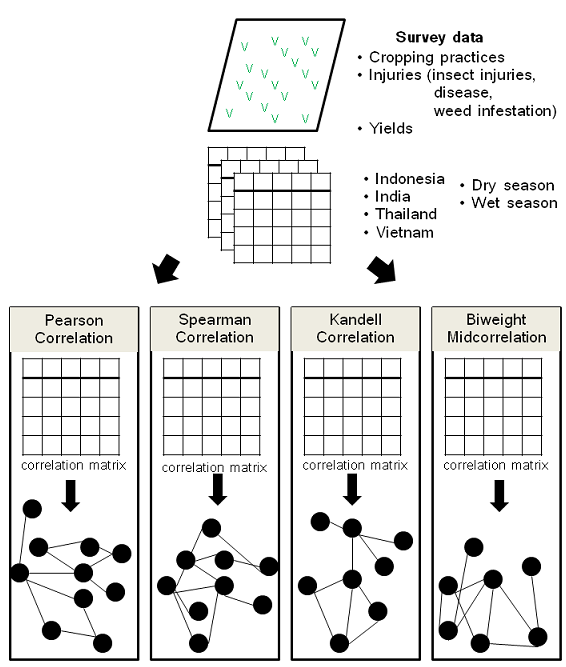
\includegraphics[resolution = 600]{pipeline}
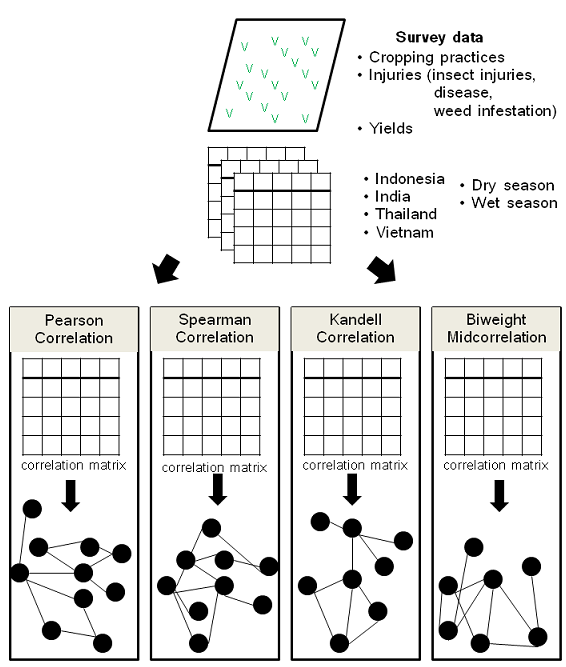
\includegraphics[width = 6in]{pipeline}
% What is FDR correction? A caption should enable a figure to stand on its own.
\caption[Network method for characterizing interactions between injury profiles and cropping practices using correlation measures]{Crop health survey data that were collected include cropping practices, injuries, and yield data. These data were collected from farmers' fields in four countries: Indonesia, India, Thailand, and Vietnam. Correlation matrices will be produced using four individual methods; Pearson, Spearman, Kendall correlation and Biweight midcorrelation. The $p$~values for all coefficients will be adjusted for multiple comparison by false discovery rate (FDR) correction. The correlation coefficients with $p$~values > 0.05 will be removed. The resulting network will be analyzed for structural properties and to infer biological meanings. This will provide the cropping practices and injury profiles network of crop health data.}
\end{figure}
%\end{landscape}

\newpage
\begin{landscape}
\begin{figure}
\centering
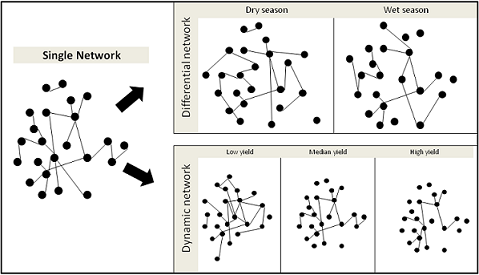
\includegraphics[width=8in]{wholenet}
\caption[Network comparison]{A single network will be created from the whole survey data set. Differential networks will be constructed using different data set, which may be different subgroups of samples from different seasons (\textit{e.g.}, dry season and wet season) or different geographic locations, then differences in connectivity patterns between two networks will be measured. Dynamic networks will be produced from different subgroups of surveys by grouping consecutive yield levels, (\textit{i.e.}, low, median, high yield).}
\end{figure}
\end{landscape}

%================eos================================

%=============================================
% CONCLUSION
%\chapter{Conclusion}
%==============================================
%%===================
% CONCLUSION
%===================
To manage broad range of pests in sustainable way of agriculture, understandings of yield constrains are required priority. Agroecosystems are diverse and complex. Networks are commonly applied to analyze systemic interplay of biological components. Network analysis enables us to the explore the complex biological process and understand holistically. The gene-gene interaction networks, for instance, reveal the gene functions and system. Besides, the emergence properties after network reconstruction give the clues to cluster the components that close related, called hub. Networks are not static when different environment can reprogram the components arrangements and functions. Moreover, networks can allow us the consider the only the elements response the given changes. With versatile applications of network analysis, agroecosystem potentially can be modeled as a network. The new type of information will be proposed from the network analysis. One of the most challenge will be the model evaluation. Because this is the first attempt to applied network into the context of rice agroecosystem. Meeting this goal will require the development the validated methods to integrate heterogeneous data and built different networks on the basis of the particular rice agroecosystem.   




% The \appendix statement indicates the beginning of the appendices.

%----------------------------------------------------------------------
% END MATERIAL
%----------------------------------------------------------------------

% B I B L I O G R A P H Y
% -----------------------

\renewcommand{\bibname}{LITERATURE CITED}
\bibliographystyle{apacite}
\bibliography{reference}
\end{document}
`